\section{Overview}

\begin{figure}
  \centering
  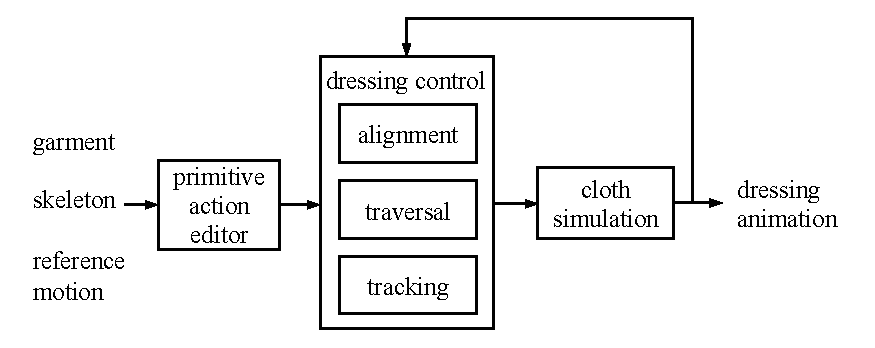
\includegraphics[width=3.3in]{images/overview}
  \caption{The overview of our system.}
\karen{The arrow heads are too thick.}
  \label{fig:overview}
\end{figure}

\begin{table}
  \centering
  \begin{tabular}{|l|l|}
    \hline
    Action & Description \\
    \hline
    Grip(RH, $\vc{f}_{1}$) & Grip the collar feature $\vc{f}_1$  with the right hand.\\
    Track($\hat{\vc{q}}(t)$, $T_1$) & Track the reference motion $\hat{\vc{q}}$ for $T_1$ seconds.\\
    Align(LH, $\vc{f}_{2}$) & Align the left hand with the armhole $\vc{f}_2$.\\
    Drag(RH, $\{B_i\}$) & Drag the cloth along the left hand $B_1$, the left\\
    &                      arm $B_2$ and the left shoulder $B_3$.\\
    Release(RH) & Release the cloth from the right hand.\\
    Track($\hat{\vc{q}}$(t), $T_2$) & Track the reference motion $\hat{\vc{q}}$ for $T_2$ seconds.\\
    Align(RH, $\vc{f}_{3}$) & Align the right hand with the right armhole $\vc{f}_3$.\\
    Stretch(RH) & Stretching the right hand into the sleeve.\\
    Track($\hat{\vc{q}}$(t), $T_3$) & Track the reference motion $\hat{\vc{q}}$ for $T_3$ seconds. \\
    Idle($T_4$) & Idle for $T_4$ seconds.\\
    \hline
  \end{tabular}
  \caption{An example action queue for dressing the upper body of a character with a jacket.}
  \label{table:actionQueue}
\end{table}


We have designed a system that allows a virtual human character to put on
various types of garments. Our system consists of three main components:
the primitive action editor, the dressing controller and the cloth
simulator. The input to our system includes a garment, a character, and a
reference dressing motion that approximates the desired dressing style.
The reference motion can be a motion captured sequence or a sparse set of
keyframes. The user first assembles a sequence of actions to describe the
reference motion using our primitive action editor. For example, putting
an arm into a sleeve can be described as first \emph{aligning} the hand
with the armhole and then \emph{dragging} the cloth up the arm, from the
wrist to the shoulder. These primitive actions are parameterized
building blocks for creating various dressing animations.
Table~\ref{table:actionQueue} shows a complete action queue for putting on
a jacket. At each step, our system fetches an action from the
queue, executes the corresponding dressing controller and simulates the
physics of the cloth. Figure \ref{fig:overview} illustrates the main
components of our system. 


